\documentclass{oblivoir}
\usepackage{amsmath,amssymb,amsthm,kotex,paralist,kswrapfig}

\usepackage[skipabove=10pt,skipbelow=10pt,innertopmargin=10pt]{mdframed}

\usepackage{tabto,pifont}
\TabPositions{0.2\textwidth,0.4\textwidth,0.6\textwidth,0.8\textwidth}
\newcommand\tabb[5]{\par\bigskip\noindent
\ding{172}\:{\ensuremath{#1}}
\tab\ding{173}\:\:{\ensuremath{#2}}
\tab\ding{174}\:\:{\ensuremath{#3}}
\tab\ding{175}\:\:{\ensuremath{#4}}
\tab\ding{176}\:\:{\ensuremath{#5}}}

\usepackage{enumitem}
\setlist[enumerate]{label=(\arabic*)}

\newcounter{num}
\newcommand{\defi}[1]
{\noindent\refstepcounter{num}\textbf{정의 \arabic{num}) #1}\par\noindent}
\newcommand{\theo}[1]
{\noindent\refstepcounter{num}\textbf{정리 \arabic{num}) #1}\par\noindent}
\newcommand{\exam}[1]
{\bigskip\bigskip\noindent\refstepcounter{num}\textbf{예시 \arabic{num}) #1}\par\noindent}
\newcommand{\prob}[1]
{\bigskip\bigskip\noindent\refstepcounter{num}\textbf{문제 \arabic{num}) #1}\par\noindent}
\newcommand{\proo}
{\bigskip\textsf{증명)}\par}

\newcommand{\ans}{
{\par\raggedleft\textbf{답 : (\qquad\qquad\qquad\qquad\qquad\qquad)}\par}\bigskip\bigskip}
\newcommand\an[1]{\par\bigskip\noindent\textbf{문제 #1)}\\}

\newcommand{\pb}[1]%\Phantom + fBox
{\fbox{\phantom{\ensuremath{#1}}}}

\newcommand\ba{\,|\,}

\let\oldsection\section
\renewcommand\section{\clearpage\oldsection}

\newenvironment{talign}
 {\let\displaystyle\textstyle\align}
 {\endalign}
\newenvironment{talign*}
 {\let\displaystyle\textstyle\csname align*\endcsname}
 {\endalign}

%%%%
\begin{document}

\title{민형 : 03 정적분}
\author{}
\date{\today}
\maketitle
\tableofcontents
\newpage

%%
\section{정적분의 정의와 미적분의 기본정리}

\begin{mdframed}
%
\defi{정적분의 정의}
함수 \(f(x)\)가 \([a,b]\)에서 연속일 때, 그래프 \(y=f(x)\)와 \(x\)축 사이의 넓이를 `구간 \([a,b]\)에서 \(f\)의 \textbf{정적분}'이라고 부르고 기호로
\[\int_a^bf(x)\,dx\]
라고 쓴다.
\end{mdframed}

\begin{figure*}[h!]
\centering
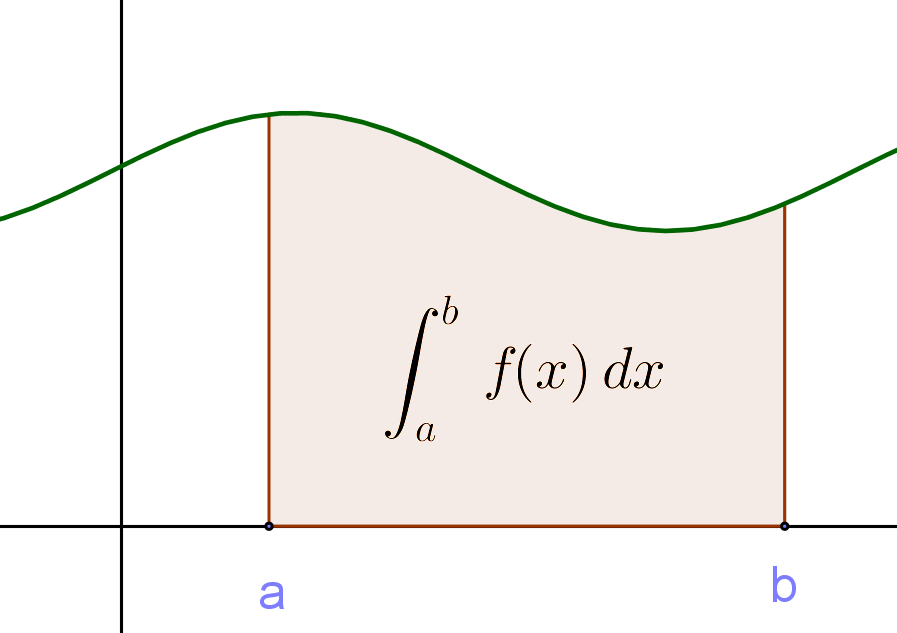
\includegraphics[width=0.4\textwidth]{area}
\end{figure*}

\begin{enumerate}
\item
구간 \([a,b]\)에서, \(f(x)>0\)이면 정적분값은 양수이고  \(f(x)<0\)이면 정적분값은 음수이다.
\item
이때 \(a\)를 \textbf{아래끝}, \(b\)를 \textbf{위끝}, \(f(x)\)를 \textbf{피적분함수}, \(x\)를 \textbf{적분변수}라고 부른다.
\item
구분구적법을 이용하면
\[\int_a^bf(x)\,dx=\lim_{n\to\infty}\sum_{k=1}^nf\left(a+\frac{b-a}nk\right)\frac{b-a}n\]
라는 관계식을 얻을 수도 있다.
\item
\[\int_b^af(x)\,dx=-\int_a^bf(x)\,dx,\]
\[\int_a^bf(x)\,dx+\int_b^cf(x)\,dx=\int_a^cf(x)\,dx\]
와 같은 성질을 가진다.
\end{enumerate}

\clearpage
정적분을 계산할 때에는 피적분함수의 부정적분에 위끝과 아래끝을 넣어 그 차를 구한다;
\begin{mdframed}
%
\defi{미적분의 기본 정리}
\(f(x)\)의 한 부정적분을 \(F(x)\)라고 하면 다음이 성립한다.
\[\int_a^bf(x)\,dx=F(b)-F(a).\]
\end{mdframed}
우변의 \(F(b)-F(a)\)는
\[\Big[F(x)\Big]_a^b,\quad\Big[F(x)\Big]_{x=a}^{x=b}\]
와 같이 표현하기도 한다.

%
\exam{}
\begin{enumerate}
\item
\(\displaystyle\int_1^2\frac{2x+1}{x^2}\,dx
=\int_1^2\left(\frac2x+x^{-2}\right)\,dx
=\left[2\ln|x|-\frac1x\right]_1^2
=2\ln2+\frac12\)
\item
\(\displaystyle
\int_0^{\frac\pi3}\tan^2x\,dx
=\int_0^{\frac\pi3}\left(\sec^2x-1\right)\,dx=\left[\tan x-x\right]_0^{\frac\pi3}
=\sqrt3-\frac\pi3
\)
\end{enumerate}

%
\prob{}
(1)\:\:
\(\displaystyle\int_1^4\left(\sqrt x-\frac2x\right)\,dx\)
\tabto{0.5\textwidth}
(2)\:\:
\(\displaystyle\int_0^\pi\cos^2x\,dx\)
\begin{mdframed}
\vspace{0.25\textheight}
\end{mdframed}
{\par\raggedleft\textbf{답 : (1) \(\frac{14}3-4\ln2\),\quad(2) \(\frac\pi2\)}\par}\bigskip

%%
\section{정적분의 치환적분법}
\begin{mdframed}
%
\theo{치환적분법}
\(t=g(x)\)일 때,
\[\int_a^bf(g(x))g'(x)\,dx=\int_{g(a)}^{g(b)}f(t)\,dt\]
\end{mdframed}
\proo
\(f(t)\)의 부정적분을 \(F(t)\)라고 하면 \(f(g(x))g'(x)\)의 부정적분은
\[\int f(g(x))g'(x)\,dx=F(g(x))+C\]
이므로 
\begin{align*}
\int_a^bf(g(x))g'(x)\,dx
&=\big[F(g(x))\big]_{x=a}^{x=b}\\
&=F(g(b))-F(g(a))\\
&=\big[F(t)\big]_{t=g(a)}^{t=g(b)}\\
&=\int_{g(a)}^{g(b)}f(t)\,dt
\end{align*}
\qed

%
\exam{}
\begin{enumerate}
\item
\(\displaystyle\int_0^1\frac{x}{(x^2+1)^2}\,dx\)
\par\bigskip\noindent
\(t=x^2+1\)이라고 하면 \(\frac{dt}{dx}=2x\)이다.
따라서
\begin{align*}
\int_0^1\frac{x}{(x^2+1)^2}\,dx
&=\frac12\int_0^1\frac1{(x^2+1)^2}\cdot 2x\,dx
=\frac12\int_0^1\frac1{t^2}\cdot\frac{dt}{dx}\,dx\\
&=\frac12\int_1^2t^{-2}\,dt=\frac12\big[-t^{-1}\big]_1^2\\
&=\frac12\left[\left(-\frac12\right)-(-1)\right]=\frac14.
\end{align*}
\item
\(\displaystyle\int_0^{\frac\pi2}\frac{\cos x}{1+2\sin x}\,dx\)
\par\bigskip\noindent
\(t=1+2\sin x\)이라고 하면 \(\frac{dt}{dx}=2\cos x\)이다.
따라서
\begin{align*}
\int_0^{\frac\pi2}\frac{\cos x}{1+2\sin x}\,dx
&=\frac12\int_0^{\frac\pi2}\frac1{1+2\sin x}\cdot2\cos x\,dx
=\frac12\int_0^{\frac\pi2}\frac1t\cdot\frac{dt}{dx}\,dx\\
&=\frac12\int_1^3\frac1t\,dx
=\frac12\Big[\ln|t|\Big]_1^3=\frac12\ln 3.
\end{align*}
\end{enumerate}

%
\prob{}
\par\noindent
(1)\:\:
\(\displaystyle\int_{\ln2}^1\frac1{e^x-e^{-x}}\,dx\)
\tabto{0.5\textwidth}
(2)\:\:
\(\displaystyle\int_1^e\frac{(\ln x)^2}x\,dx\)
\par\vspace{10pt}\noindent
(3)\:\:
\(\displaystyle\int_2^7\frac x{\sqrt{x+2}}\,dx\)
\tabto{0.5\textwidth}
(4)\:\:
\(\displaystyle\int_1^e\ln\sqrt[x]x\,dx\)
\par\vspace{10pt}\noindent
(5)\:\:
\(\displaystyle\int_0^{\frac\pi6}(1-\sin^2x)\cos x\,dx\)
\tabto{0.5\textwidth}
(6)\:\:
\(\displaystyle\int_0^{\frac\pi2}\frac{\sin^3x}{1+\cos x}\,dx\)
\begin{mdframed}
\vspace{0.3\textheight}
\end{mdframed}
{\par\raggedleft\textbf{답 : }
(1) \(\frac12\ln\frac{3(e-1)}{e+1}\),\quad
(2) \(\frac13\),\quad
(3) \(\frac{26}3\),\quad
(4) \(\frac12\),\quad
(5) \(\frac{11}{24}\),\quad
(6) \(\frac12\)
\par}\bigskip

\clearpage
%
\exam{}
\begin{enumerate}
\kswrapfig[Pos=r,Width=4cm]{2sinx}{
\item
\(\displaystyle\int_0^2\sqrt{4-x^2}\,dx\)
\par\bigskip\noindent
\(x=2\sin\theta\) (\(-\frac\pi2\le\theta\le\frac\pi2)\)
로 놓으면
\begin{align*}
\sqrt{4-x^2}
&=\sqrt{4-4\sin^2\theta}=2\sqrt{1-\sin^2\theta}\\
&=2|\cos\theta|=2\cos\theta
\end{align*}
이고
\(dx=2\cos\theta d\theta\)이다.
따라서}
\begin{align*}
\int_0^2\sqrt{4-x^2}\,dx
&=\int_0^{\frac\pi2}2\cos\theta\cdot2\cos\theta\,d\theta
=4\int_0^{\frac\pi2}\cos^2\theta\,d\theta\\
&=4\int_0^{\frac\pi2}\frac{1+\cos 2\theta}2\,d\theta
=2\left[\theta+\frac12\sin2\theta\right]_0^{\frac\pi2}=\pi
\end{align*}
\kswrapfig[Pos=r,Width=3cm]{2tanx}{
\item
\(\displaystyle\int_0^2\frac1{4+x^2}\,dx\)
\par\bigskip\noindent
\(x=2\tan\theta\) (\(-\frac\pi2<\theta<\frac\pi2)\)
로 놓으면
\[\frac1{4+x^2}=\frac1{4+4\tan^2\theta}=\frac1{4\sec^2\theta}=\frac14\cos^2\theta\]이고
\(dx=2\sec^2\theta\,d\theta\)이다.
따라서}
\begin{align*}
\int_0^2\frac1{4+x^2}\,dx
&=\int_0^2\frac1{4+x^2}\,dx
=\int_0^{\frac\pi4}\frac14\cos^2x\cdot2\sec^2\theta\,d\theta\\
&=\int_0^{\frac\pi4}\frac12\,d\theta
=\left[\frac12\theta\right]_0^{\frac\pi4}=\frac\pi8
\end{align*}
\end{enumerate}
%
\prob{}
\par\noindent
(1)\:\:
\(\displaystyle\int_0^3\sqrt{9-x^2}\,dx\)
\tabto{0.33\textwidth}
(2)\:\:
\(\displaystyle\int_0^{\frac12}\frac1{\sqrt{1-x^2}}\,dx\)
\tabto{0.66\textwidth}
(3)\:\:
\(\displaystyle\int_{-\sqrt3}^{\sqrt3}\frac1{x^2+9}\,dx\)
\begin{mdframed}
\vspace{0.3\textheight}
\end{mdframed}
{\par\raggedleft\textbf{답 : }
(1) \(\frac94\pi\),\quad
(2) \(\frac\pi6\),\quad
(3) \(\frac\pi9\)
\par}\bigskip

%%
\section{정적분의 부분적분법}
\begin{mdframed}
%
\theo{부분적분법}
\[\int_a^bf(x)g'(x)\,dx=\Big[f(x)g(x)\Big]_a^b-\int_a^bf'(x)g(x)\,dx\]
\end{mdframed}
\proo
\begin{align*}
\Big[f(x)g(x)\Big]_a^b
&=\int_a^b\left\{f(x)g(x)\right\}'\,dx\\
&=\int\left(f(x)g'(x)+f'(x)g(x)\right)\,dx\\
&=\int_a^bf(x)g'(x)\,dx+\int_a^bf'(x)g(x)\,dx\\
\end{align*}
이므로 이를 변형하면 위의 결과를 얻는다.
\qed

%
\exam{}
\par\noindent
\(\displaystyle\int_0^{\frac\pi2}x\cos x\,dx\)를 계산하기 위해 \(f(x)=x\), \(g'(x)=\cos x\)라고 하자.
\(f'(x)=1\), \(g(x)=\sin x\)이므로
\begin{align*}
\int_0^{\frac\pi2}x\cos x\,dx
&=\int_0^{\frac\pi2}f(x)g'(x)\,dx\\
&=\left[f(x)g(x)\right]_0^{\frac\pi2}-\int_0^{\frac\pi2}f'(x)g(x)\,dx\\
&=\left[x\sin x\right]_0^{\frac\pi2}-\int_0^{\frac\pi2}\sin x\,dx\\
&=\frac\pi2-\left[-\cos x\right]_0^{\frac\pi2}=\frac\pi2-1
\end{align*}
\end{document}